\documentclass[11pt,a4paper]{article}

\usepackage[utf8]{inputenc}
\usepackage[T1]{fontenc}
\usepackage[french]{babel}
\usepackage{lmodern}
\usepackage{geometry}
\geometry{margin=2.3cm}
\usepackage{graphicx}
\usepackage{booktabs}
\usepackage{multirow}
\usepackage{amsmath,amssymb}
\usepackage{xcolor}
\usepackage{enumitem}
\usepackage{caption}
\usepackage[hidelinks]{hyperref}
\captionsetup{font=small,labelfont=bf}

\newcommand{\best}[1]{\textbf{#1}}

\title{\textbf{Modèle CLIP ARN--protéine et niches spatiales multi-omiques}\\[4pt]
\large Méthodologie, résultats et analyses --- rapport détaillé}
\author{Louise Lapie --- CDD (6 mois)}
\date{Juin 2026 \quad(document de travail pour la présentation du 9 juillet 2026)}

\begin{document}
\maketitle

\begin{abstract}
\noindent
Ce rapport documente un modèle contrastif (CLIP) alignant, pour des cellules
\emph{strictement appariées}, une vue \textbf{transcriptomique} (ARN) et une vue
\textbf{protéomique} (protéine), sur deux jeux de données de transcriptomique spatiale
sub-cellulaire : \textbf{CosMx} (sein, 64 marqueurs protéiques) et \textbf{Xenium}
(rein, 27 marqueurs). À partir des embeddings cellulaires du modèle, on calcule des
\textbf{niches spatiales} en réutilisant la « fin de NOVAE » (projection sur la sphère,
prototypes, transport optimal, clustering hiérarchique). On compare plusieurs encodeurs
ARN (NOVAE \emph{vs} scConcept) et plusieurs espaces (ARN seul, protéine seule,
multi-omique) selon : la continuité spatiale (FIDE), le recouvrement avec les types
cellulaires, une analyse d'\emph{information} (variance expliquée), et surtout une
\textbf{validation contre des annotations de pathologie} (vérité terrain, Xenium).
Le message principal : \textbf{NOVAE produit de vraies niches spatiales} là où scConcept
produit surtout du typage cellulaire ; et \textbf{l'intégration multi-omique apporte un
signal protéique réel}, retrouvant mieux l'histologie que chaque modalité prise seule.
L'avantage reste toutefois \textbf{compétitif plutôt que décisif} une fois la baseline
ARN fortement entraînée (NOVAE fine-tuné), ce qui motive les expériences à venir.
\end{abstract}

\tableofcontents
\bigskip

%==============================================================
\section{Contexte et objectif}
%==============================================================
La transcriptomique spatiale conserve la position des cellules, ce qui permet d'étudier
les \emph{micro-environnements} (ou \textbf{niches} / domaines spatiaux). Le projet vise
à entraîner un premier modèle \textbf{CLIP-like} qui apprend un espace commun entre l'ARN
et la protéine de cellules appariées, puis à se demander :
\begin{enumerate}[noitemsep]
  \item l'embedding \emph{multi-omique} produit-il de \emph{meilleures niches} que chaque
        modalité seule ?
  \item quel encodeur ARN gelé vaut-il mieux donner au CLIP : \textbf{NOVAE} (conscient du
        voisinage spatial) ou \textbf{scConcept} (par cellule) ?
\end{enumerate}
Un constat de départ oriente toute l'étude : au \emph{retrieval} cross-modal (retrouver la
protéine d'une cellule à partir de son ARN), \textbf{scConcept bat NOVAE}
(R@5 moyen sur CosMx : $\approx$2{,}6\,\% pour scConcept contre $\approx$0{,}7\,\% pour
NOVAE). Le retrieval est une métrique \emph{cellule-à-cellule}. La question devient alors :
est-ce que cet avantage s'inverse au niveau \emph{voisinage}, c'est-à-dire pour les niches ?

%==============================================================
\section{Données}
%==============================================================
\begin{table}[h]
\centering
\small
\begin{tabular}{lccccc}
\toprule
Jeu & Tissu & Cellules & Gènes (ARN) & Marqueurs prot. & Annotations \\
\midrule
CosMx  & sein & 152\,446 & $\sim$20\,000 & 64 & types cell.$^\dagger$ \\
Xenium & rein & 465\,498 & 405 & 27 & types cell.$^\dagger$ + \textbf{pathologie} \\
\bottomrule
\end{tabular}
\caption{Les deux jeux de données. Chaque cellule possède une vue ARN \emph{et} une vue
protéine (même cellule). Coordonnées spatiales (µm) disponibles. Le Xenium dispose
en plus d'\textbf{annotations de pathologie} (régions tracées par un pathologiste sur le
H\&E, alignées sur les cellules).
$^\dagger$ \emph{Les annotations de types cellulaires ont été produites par nous-mêmes par
label transfer scConcept --- ce ne sont donc pas des annotations de référence externes.
Seule la pathologie (Xenium) est une vérité terrain externe.}}
\end{table}

\noindent
\textbf{Splits.} Un découpage spatial train/val/test/buffer existe pour l'entraînement
supervisé du CLIP (le \emph{retrieval} s'évalue sur le test tenu à l'écart). La découverte
de niches étant \emph{non supervisée}, elle utilise la lame entière (aucune fuite d'étiquette).

%==============================================================
\section{Méthodologie}
%==============================================================

\subsection{Modèle CLIP ARN--protéine}
Deux « tours » projettent chaque modalité dans un espace commun de dimension 256,
normalisé L2 :
\begin{itemize}[noitemsep]
  \item \textbf{Tour ARN} : embedding gelé (NOVAE 64d \emph{ou} scConcept 512d, précalculé)
        $\rightarrow$ \texttt{Linear}$\rightarrow$ L2 $\;=\; z_r$.
  \item \textbf{Tour protéine} : intensités prétraitées (clip 1--99, $\log(1+x)$, z-score par
        marqueur, ajusté sur le train) $\rightarrow$ MLP $\rightarrow$ L2 $\;=\; z_p$.
\end{itemize}
Loss \textbf{InfoNCE symétrique} (température 0{,}07) : la paire positive de la ligne $i$ est
la colonne $i$. On obtient, par cellule, $z_r$ et $z_p$, et la \textbf{fusion multi-omique}
$z_{\text{joint}} = \mathrm{L2}(z_r + z_p)$.

\subsection{Tête de niches : la « fin de NOVAE »}
On réutilise la partie inférence (zero-shot) de NOVAE\footnote{Blampey \emph{et al.},
\emph{Novae: a graph-based foundation model for spatial transcriptomics data},
Nature Methods 22:2539--2550 (2025).} appliquée à des embeddings \emph{quelconques}
(module \texttt{src/niches.py}) :
\begin{enumerate}[noitemsep]
  \item projection sur la \textbf{sphère unité} (L2) ;
  \item \textbf{prototypes} = $K{=}512$ centres de KMeans sur les embeddings normalisés ;
  \item \textbf{attribution} d'un prototype « feuille » par cellule (argmax cosinus ;
        variante transport optimal / Sinkhorn disponible) ;
  \item \textbf{clustering hiérarchique} (cosine, average) des prototypes $\rightarrow$ arbre
        coupé à \texttt{n\_domains} domaines (= niches).
\end{enumerate}
\emph{Nuance importante :} le transport optimal sert dans NOVAE à l'\textbf{entraînement}
(cible de la loss SwAV) ; à l'\textbf{inférence}, l'attribution se fait par argmax cosinus.
Les embeddings du CLIP étant déjà L2-normalisés, l'étape « sphère » est neutre pour eux ;
ce que NOVAE \emph{ajoute} réellement, c'est la machinerie prototypes $\rightarrow$
hiérarchie, pas la normalisation.

\subsection{Espaces d'embeddings comparés}
\begin{center}
\small
\begin{tabular}{ll}
\toprule
\texttt{novae\_raw} & embedding NOVAE gelé (64d) --- \emph{ARN seul, $\approx$ NOVAE zero-shot} \\
\texttt{clip\_rna}  & $z_r$ (256d) --- vue ARN projetée par le CLIP \\
\texttt{clip\_prot} & $z_p$ (256d) --- vue protéine projetée par le CLIP \\
\texttt{clip\_joint}& $\mathrm{L2}(z_r{+}z_p)$ (256d) --- \textbf{multi-omique} \\
\texttt{scconcept\_*}& idem mais encodeur ARN scConcept (512d) \\
\bottomrule
\end{tabular}
\end{center}
Tous les espaces sont évalués sur le \textbf{même graphe spatial} (kNN, $k{=}6$) pour une
comparaison équitable.

\subsection{Métriques d'évaluation}
\begin{description}[noitemsep,leftmargin=1.4em]
  \item[\textbf{FIDE}] F1 des arêtes intra-domaine. \emph{Haut} = niches spatialement
        continues (gros blocs contigus, pas du « sel-et-poivre »). \emph{Mesure la
        continuité, pas la justesse biologique.}
  \item[\textbf{Entropie normalisée}] équilibre des tailles de niches.
  \item[\textbf{Heuristique}] $=$ FIDE $\times$ entropie (compromis ; c'est le critère de
        réglage d'hyperparamètres de NOVAE).
  \item[\textbf{ARI / NMI vs types}] recouvrement des niches avec les types cellulaires.
        \emph{Bas} = niche $\neq$ type (sain : une niche est un voisinage, pas un type).
  \item[\textbf{ARI / NMI / homogénéité vs pathologie}] accord avec les régions du
        pathologiste (vérité terrain externe, Xenium). \emph{C'est la métrique la plus
        objective.}
\end{description}
\textbf{ARI vs NMI.} L'ARI raisonne sur les \emph{paires} de cellules et pénalise fort les
différences de granularité ; le NMI est informationnel et tolère mieux qu'une partition
soit plus fine que l'autre. On rapporte les deux.

\subsection{Analyse d'information (variance expliquée)}
Pour tester si une partition « contient de l'information » sur une modalité, on mesure la
\textbf{variance expliquée} ($\eta^2$) : $\mathrm{EV} = 1 - \mathrm{SS}_{\text{intra}}/
\mathrm{SS}_{\text{total}}$. Haut = les cellules d'une même niche se ressemblent dans cette
modalité. Cible protéine = intensités brutes ; cible ARN = \textbf{comptages bruts}
(indépendants), pour éviter la circularité (la jointe contient déjà l'ARN NOVAE). Un test
de \textbf{permutation} (drill-down) vérifie que les sous-divisions d'une niche ARN par la
jointe correspondent à de \emph{vraies} différences de protéine.

\subsection{Validation pathologie (Xenium)}
Le pathologiste a tracé 9 régions sur le H\&E (Tumor$\times$3, Necrosis, Immune cells,
Immune infiltration, Hemorrhage, Adipose, Blood vessels), exportées en GeoJSON. Une matrice
affine $3\times3$ (\emph{image alignment}) ramène ces polygones dans le repère µm des
cellules ; on assigne chaque cellule à sa région (point-dans-polygone). Le bon sens de la
transformation a été déterminé \emph{empiriquement} puis confirmé biologiquement
(\textbf{Tumor}$\rightarrow$32\,\% malignes, \textbf{Immune cells}$\rightarrow$33\,\% T +
17\,\% B). 92\,\% des cellules tombent dans une région annotée.

\subsection{Baselines et benchmark}
Pour situer le multi-omique face à des méthodes de domaines spatiaux (module
\texttt{benchmark/}) :
\begin{itemize}[noitemsep]
  \item \textbf{NOVAE zero-shot} ($=$\texttt{novae\_raw}) et \textbf{NOVAE fine-tuné}
        (ré-entraîné quelques epochs sur la lame, auto-supervisé) --- ARN seul ;
  \item \textbf{BANKSY-style} (propre + moyenne du voisinage, $\lambda$-pondéré, KMeans) ---
        sur ARN \emph{et} sur protéine ;
  \item \textbf{Cellular Neighborhoods} (Schürch 2020 : phénotypes protéiques
        $\rightarrow$ composition du voisinage $\rightarrow$ KMeans) --- niche \emph{protéique
        dédiée}.
\end{itemize}
\emph{Note d'honnêteté :} BANKSY-style et CN sont des versions simplifiées (sans le filtre
de Gabor azimutal de BANKSY officiel) ; suffisantes pour une première idée, à remplacer par
les packages officiels pour publication.

%==============================================================
\section{Résultats}
%==============================================================
\emph{Avertissement de cohérence :} suite aux ré-exécutions, les niches CosMx sont
rapportées à $n_{\text{dom}}{=}10$ et les niches Xenium à $n_{\text{dom}}{=}5$ ; le
\texttt{n\_domains} est précisé dans chaque table. Le balayage de la
section~\ref{sec:scan} couvre $n\in\{5,7,10,15\}$.

\subsection{Retrieval cross-modal (contexte)}
Sur le test, le CLIP \textbf{scConcept} bat le CLIP \textbf{NOVAE} (R@5 moyen CosMx
$\approx$2{,}6\,\% vs 0{,}7\,\%). Les valeurs absolues sont faibles (tâche difficile,
galerie immense), mais le \emph{classement} est net : au niveau cellulaire, scConcept porte
plus de signal fin corrélé à la protéine. C'est le point de départ : voyons les niches.

\subsection{Qualité spatiale des niches (FIDE)}
\begin{table}[h]
\centering\small
\begin{tabular}{llcccc}
\toprule
Jeu ($n$) & espace & FIDE & entropie & heuristique & NMI/types \\
\midrule
\multirow{4}{*}{CosMx (10)}
 & \texttt{novae\_raw}  & 0.599 & 0.922 & 0.552 & -- \\
 & \texttt{clip\_rna}   & 0.649 & 0.922 & 0.598 & -- \\
 & \texttt{clip\_prot}  & 0.689 & 0.846 & 0.583 & -- \\
 & \best{\texttt{clip\_joint}} & \best{0.739} & 0.846 & \best{0.625} & -- \\
\midrule
\multirow{4}{*}{Xenium (5)}
 & \texttt{novae\_raw}  & 0.815 & 0.627 & 0.511 & 0.135 \\
 & \best{\texttt{clip\_rna}} & \best{0.851} & 0.636 & 0.541 & 0.140 \\
 & \texttt{clip\_prot}  & 0.608 & 0.858 & 0.521 & 0.268 \\
 & \texttt{clip\_joint} & 0.792 & 0.811 & \best{0.642} & 0.182 \\
\bottomrule
\end{tabular}
\caption{FIDE des quatre espaces. \textbf{CosMx} (protéine riche, 64 marqueurs) :
\texttt{clip\_joint} est le meilleur en FIDE \emph{et} en heuristique. \textbf{Xenium}
(protéine mince, 27 marqueurs) : \texttt{clip\_prot} est faible (0.608) et tire la fusion
vers le bas (FIDE \texttt{clip\_joint} 0.792 $<$ \texttt{clip\_rna} 0.851) --- bien que
\texttt{clip\_joint} reste le meilleur en \emph{heuristique} (0.642) grâce à des niches plus
équilibrées. \textbf{Le bénéfice du multi-omique dépend de la richesse du panel protéique.}}
\end{table}

\subsection{NOVAE vs scConcept (niches multi-omiques)}
\begin{table}[h]
\centering\small
\begin{tabular}{llcccc}
\toprule
Jeu ($n$) & modèle & FIDE & heuristique & ARI/types & NMI/types \\
\midrule
\multirow{2}{*}{CosMx (10)} & \best{NOVAE} & \best{0.739} & \best{0.625} & 0.008 & 0.079 \\
 & scConcept & 0.503 & 0.476 & 0.033 & 0.145 \\
\midrule
\multirow{2}{*}{Xenium (5)} & \best{NOVAE} & \best{0.792} & \best{0.642} & 0.112 & 0.182 \\
 & scConcept & 0.498 & 0.462 & 0.409 & \best{0.508} \\
\bottomrule
\end{tabular}
\caption{Niches multi-omiques (\texttt{clip\_joint}) : \textbf{NOVAE bat nettement scConcept}
en continuité spatiale (FIDE) sur les deux tissus. Surtout, sur Xenium le NMI/types de
scConcept atteint \textbf{0.508} : ses « niches » sont presque une \emph{carte de types
cellulaires}, alors que NOVAE reste à 0.182 (niches distinctes des types). \textbf{NOVAE
fait des niches ; scConcept fait du typage.}}
\end{table}

\subsection{Information : multi- vs uni-omique}
\begin{figure}[h]
\centering
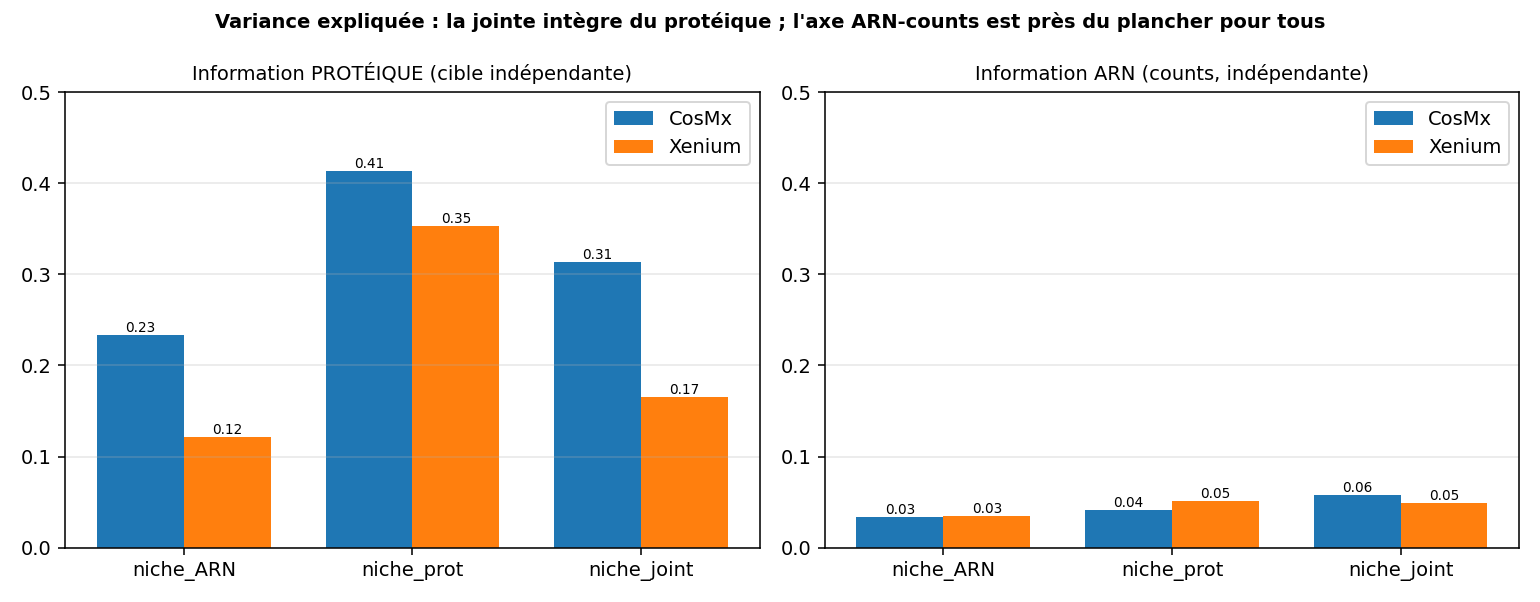
\includegraphics[width=\linewidth]{figs/info_ev_bars.png}
\caption{Variance expliquée (cibles indépendantes). \emph{À gauche} : la niche jointe
explique la protéine mieux que la niche ARN ($+0.080$ CosMx, $+0.044$ Xenium) $\rightarrow$
elle \textbf{intègre du protéique}. \emph{À droite} : l'axe ARN-comptages est près du
plancher pour \emph{toutes} les partitions (même \texttt{niche\_ARN}) --- une niche grossière
ne peut pas résumer le transcriptome cellule-à-cellule, dominé par le bruit (dropout). Ce
n'est pas une absence d'information ARN, c'est une inadéquation d'échelle.}
\end{figure}
Le \textbf{drill-down} confirme : une niche ARN scindée par la jointe donne des sous-niches
aux profils protéiques \emph{réellement} distincts (test de permutation
$p\approx0{,}005$ sur les deux tissus). \textbf{Conclusion : la protéine ajoute une
information réelle, plus marquée quand le panel est riche (CosMx).}

\subsection{Validation pathologie (Xenium) --- le résultat clé}
\label{sec:patho}
\begin{table}[h]
\centering\small
\begin{tabular}{lccc}
\toprule
méthode (clip\_joint, $n{=}10$) & ARI & NMI & homogénéité \\
\midrule
\best{NOVAE\_joint (multi-omique)} & \best{0.206} & \best{0.287} & \best{0.539} \\
NOVAE\_raw (ARN seul) & 0.112 & 0.187 & 0.348 \\
scConcept\_joint & 0.064 & 0.138 & 0.291 \\
\bottomrule
\end{tabular}
\caption{Accord avec la pathologie (vérité terrain). Le multi-omique NOVAE retrouve le
mieux les régions du pathologiste, \emph{$\approx$2$\times$} l'ARN seul, scConcept dernier.
\textbf{Important :} ce résultat \emph{nuance} le FIDE (où la fusion semblait nuire sur
Xenium) --- contre la vraie histologie, le multi-omique gagne.}
\end{table}

\begin{figure}[h]
\centering
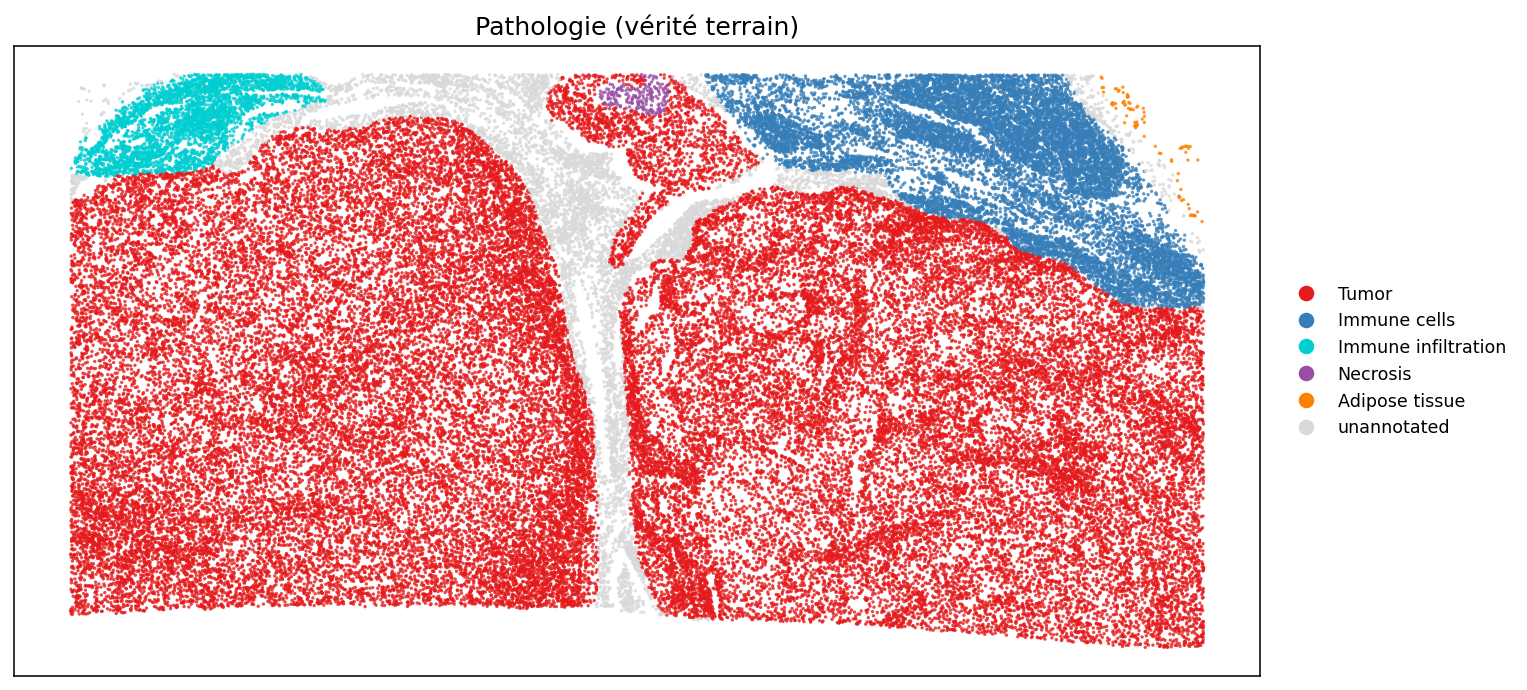
\includegraphics[width=0.32\linewidth]{figs/patho_truth.png}\hfill
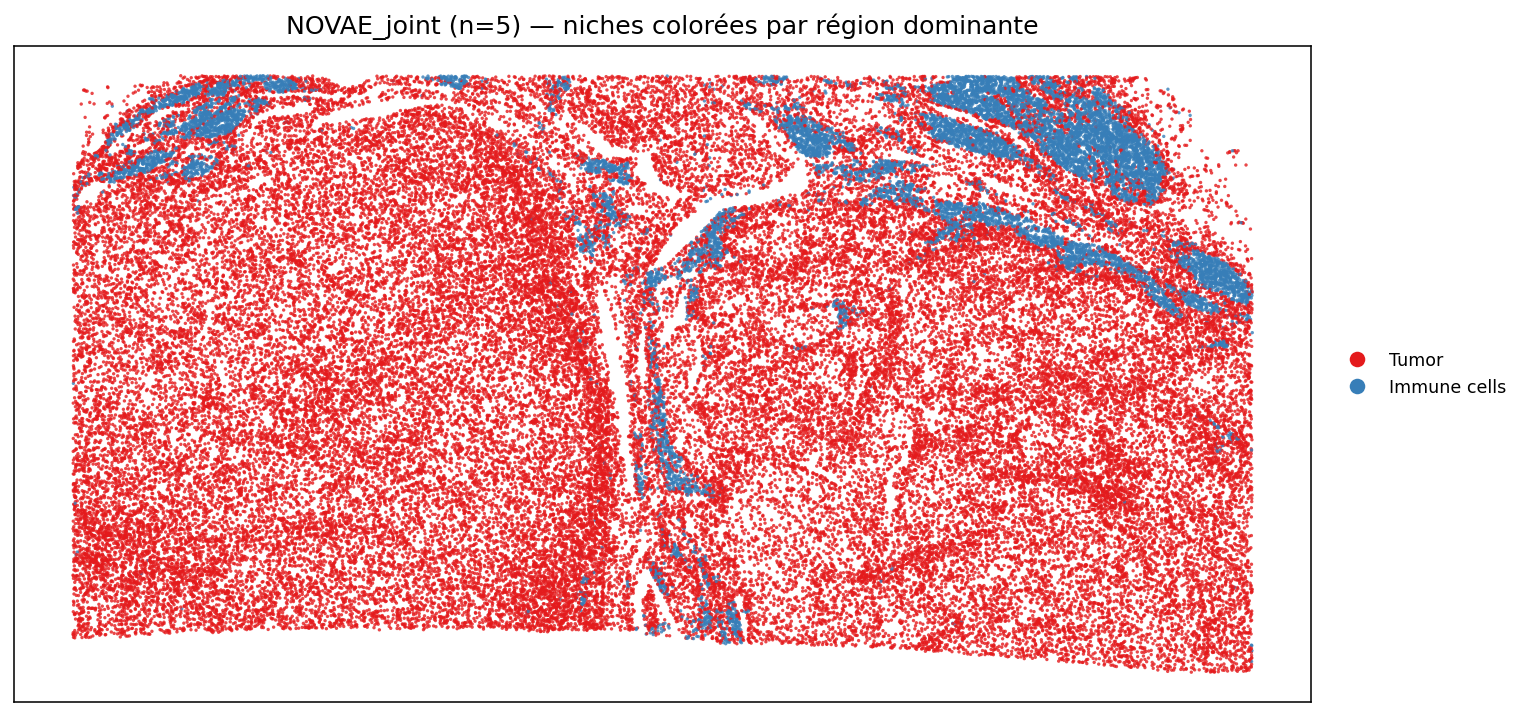
\includegraphics[width=0.32\linewidth]{figs/patho_novae_joint.png}\hfill
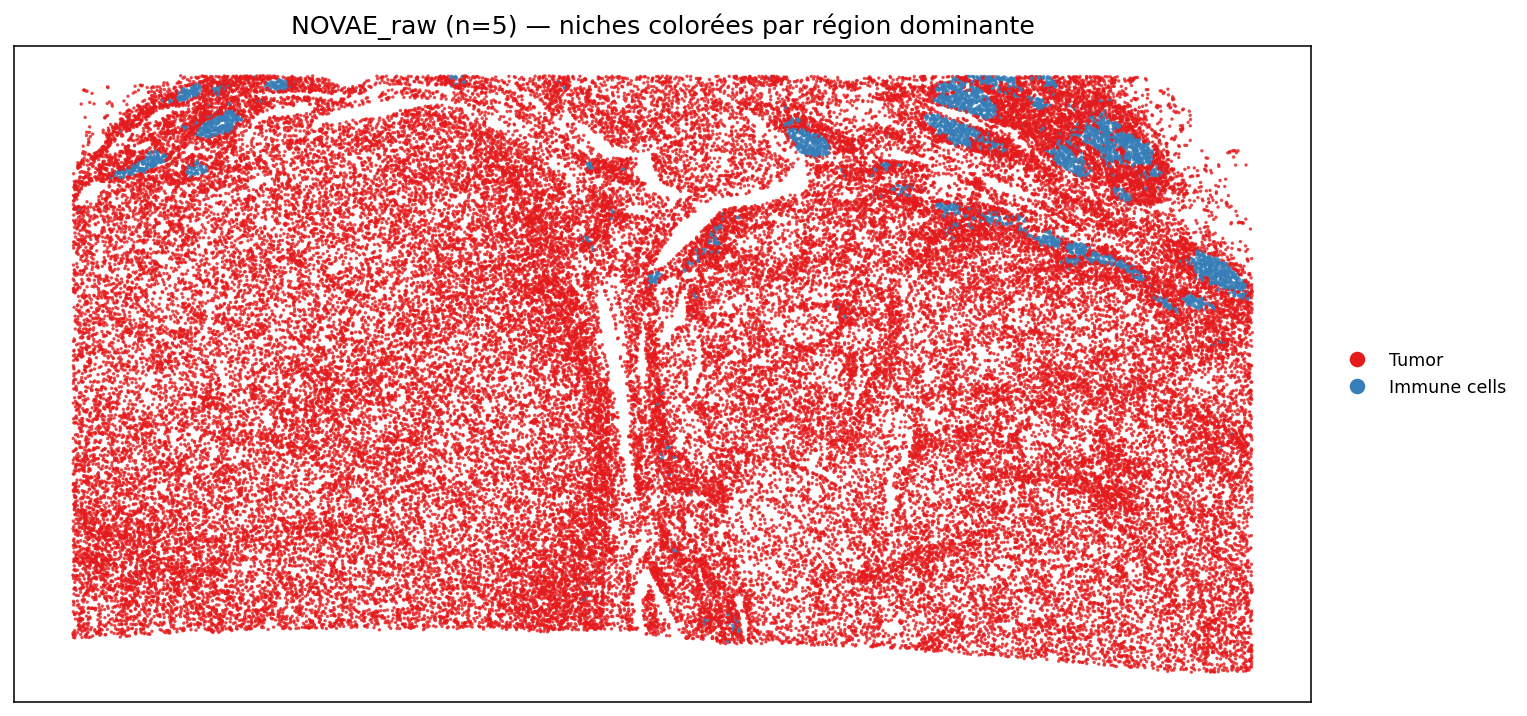
\includegraphics[width=0.32\linewidth]{figs/patho_novae_raw.png}
\caption{Cartes spatiales ($n{=}5$), même code couleur (niche colorée par sa région
dominante). De gauche à droite : \textbf{pathologie} (vérité terrain), \textbf{NOVAE\_joint}
(multi-omique), \textbf{NOVAE\_raw} (ARN seul). Le multi-omique retrouve mieux les zones
immunitaires (bleu).}
\end{figure}

\begin{figure}[h]
\centering
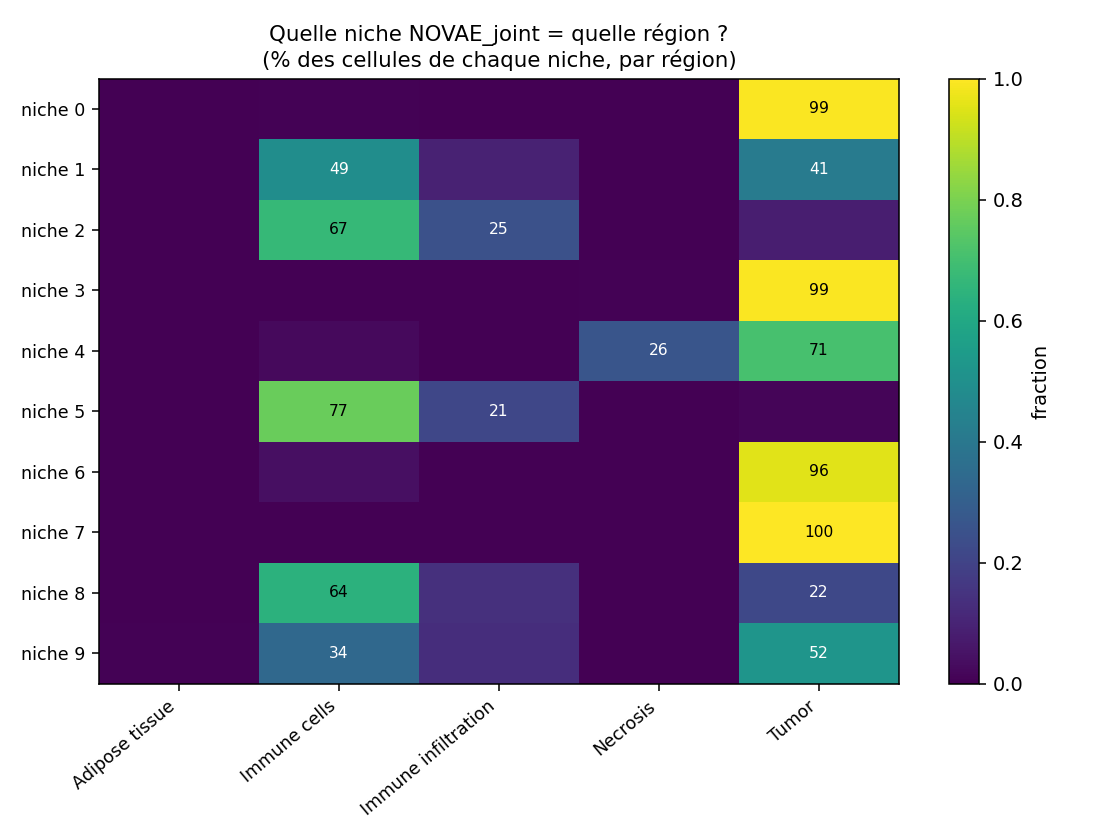
\includegraphics[width=0.62\linewidth]{figs/contingence.png}
\caption{Correspondance niche $\rightarrow$ région (NOVAE\_joint, \% des cellules de chaque
niche). Les niches 0/3/6/7 $\approx$ Tumor, 2/5/8 $\approx$ Immune ; les niches sont plus
\emph{fines} que les régions (plusieurs niches se partagent la tumeur), ce qui plafonne l'ARI.}
\end{figure}

\subsection{Robustesse au nombre de domaines}
\label{sec:scan}
\begin{table}[h]
\centering\small
\begin{tabular}{lcccc}
\toprule
ARI vs pathologie & $n{=}5$ & $n{=}7$ & $n{=}10$ & $n{=}15$ \\
\midrule
\best{NOVAE\_joint} & \best{0.426} & \best{0.414} & \best{0.206} & 0.134 \\
NOVAE\_raw          & 0.193 & 0.167 & 0.112 & 0.139 \\
scConcept\_joint    & 0.044 & 0.045 & 0.064 & 0.063 \\
\bottomrule
\end{tabular}
\caption{Balayage de $n_{\text{dom}}$. NOVAE\_joint domine à $n{=}5,7,10$ (et l'accord
\emph{absolu} est le meilleur à $n\approx5$, qui correspond au nombre de régions annotées).
À $n{=}15$ l'avantage s'efface (sur-découpage vs $\sim$5 régions grossières). \textbf{Fenêtre
à rapporter : $n{=}5$--$10$.} Choisir $n$ pour \emph{maximiser} l'accord serait un biais ;
ici on rapporte tous les $n$ (comme l'article NOVAE, qui benchmarke à 7/10/15).}
\end{table}
\begin{figure}[h]
\centering
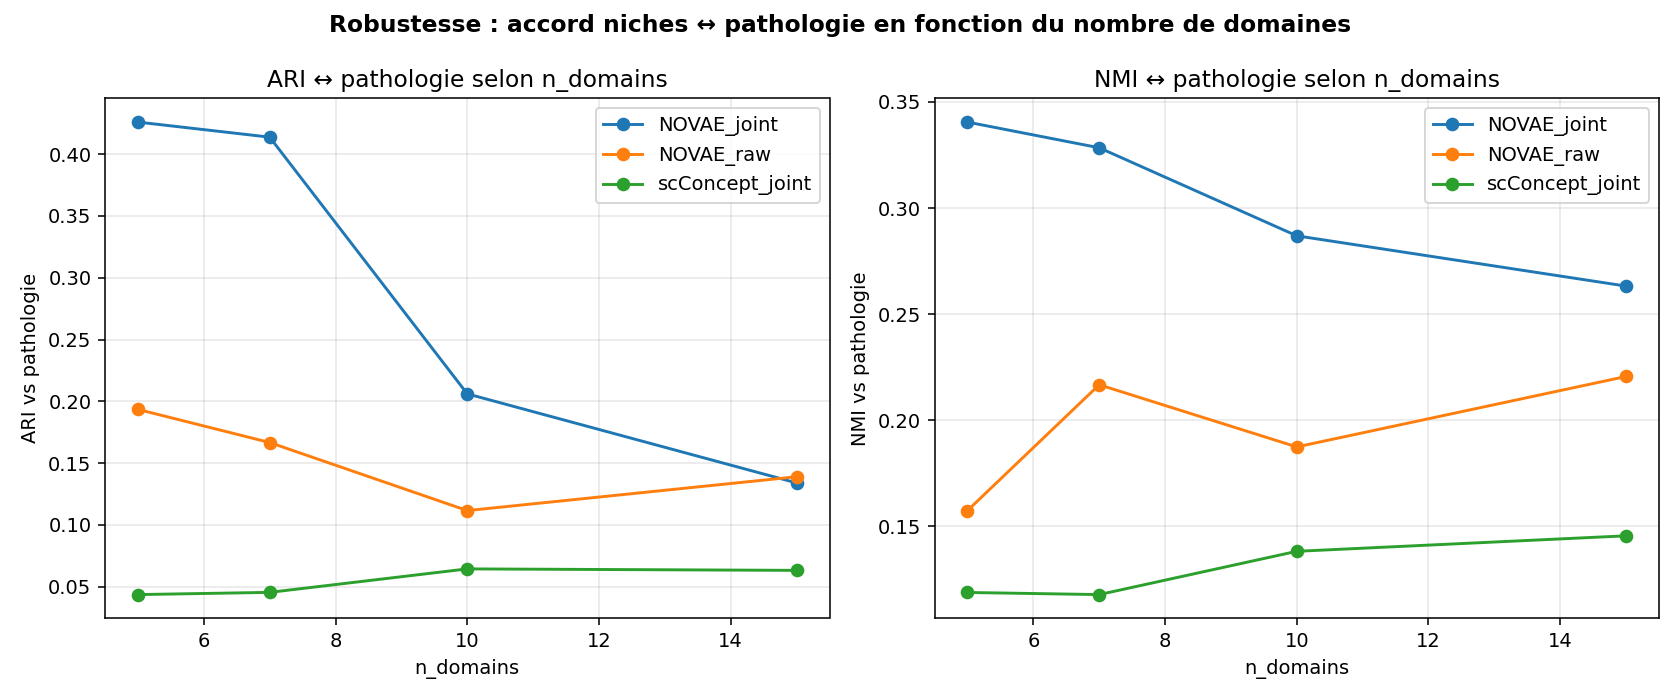
\includegraphics[width=0.9\linewidth]{figs/scan_ndomains.png}
\caption{ARI et NMI vs pathologie en fonction de $n_{\text{dom}}$ pour les trois méthodes.}
\end{figure}

\subsection{Les niches valent-elles mieux que du typage ?}
Baseline « types cellulaires seuls » vs pathologie : ARI $0.05$--$0.09$
(\texttt{cell\_type\_final} 0.051\,/\,0.077 ; \texttt{qc\_celltype\_cpu} 0.088\,/\,0.094)
--- très en dessous des niches (NOVAE\_joint 0.206). \textbf{Les niches capturent une vraie
structure spatiale, pas un recoloriage des types.}

\subsection{Benchmark vs méthodes de référence (Xenium, $n{=}5$)}
\label{sec:bench}
\begin{table}[h]
\centering\small
\begin{tabular}{llccc}
\toprule
méthode & modalité & ARI & NMI & homog. \\
\midrule
\best{NOVAE\_joint} & \best{multi-omique} & \best{0.426} & 0.341 & 0.487 \\
NOVAE fine-tuné & ARN & 0.239 & \best{0.353} & \best{0.552} \\
BANKSY-style & ARN & 0.193 & 0.278 & 0.436 \\
NOVAE zero-shot (\texttt{novae\_raw}) & ARN & 0.193 & 0.157 & 0.198 \\
Cellular Neighborhoods & protéine & 0.182 & 0.251 & 0.396 \\
BANKSY-style & protéine & 0.135 & 0.235 & 0.368 \\
scConcept\_joint & multi-omique & 0.044 & 0.119 & 0.192 \\
\bottomrule
\end{tabular}
\caption{Multi-omique vs baselines uni-modales et NOVAE fine-tuné.
\textbf{(i)} Le multi-omique bat \emph{chaque modalité seule} : ARN ($\le$0.19) et protéine
($\le$0.18) --- y compris une méthode protéique \emph{dédiée} (CN). \textbf{(ii)} Mais face
au \textbf{NOVAE fine-tuné} (baseline ARN forte), la comparaison se resserre : le
multi-omique gagne sur l'ARI (0.426 vs 0.239) mais le fine-tuné \emph{égale/dépasse} sur le
NMI (0.353 vs 0.341) et l'homogénéité. \textbf{Avantage réel mais pas décisif} une fois
l'ARN bien entraîné.}
\end{table}

%==============================================================
\section{Analyse et discussion}
%==============================================================
\begin{description}[leftmargin=1.2em]
  \item[\textbf{1. NOVAE = niches, scConcept = typage (solide).}] Sur les deux tissus,
        NOVAE donne des niches spatialement continues et distinctes des types ; scConcept
        donne des cartes qui collent aux types cellulaires (NMI/types jusqu'à 0.51 sur
        Xenium). Pour une tâche de domaines spatiaux, un encodeur conscient du voisinage est
        le bon choix --- \emph{même s'il perd au retrieval cellulaire}. C'est la dissociation
        centrale : retrieval (cellule) et niche (voisinage) mesurent des choses différentes.
  \item[\textbf{2. Le multi-omique apporte un signal protéique réel.}] Validé par
        l'analyse d'information ($p\approx0.005$) \emph{et} par la pathologie : le
        multi-omique retrouve l'histologie mieux que l'ARN seul, la protéine seule, et même
        une méthode protéique dédiée.
  \item[\textbf{3. Mais l'avantage dépend du panel et de la baseline.}] Le bénéfice FIDE
        n'apparaît que si la protéine est riche (CosMx) ; et face à un NOVAE \emph{fine-tuné}
        l'écart se resserre (métrique-dépendant). On ne peut donc pas écrire « multi-omique
        $\gg$ ARN » sans nuance.
  \item[\textbf{4. FIDE $\neq$ information $\neq$ pathologie.}] Trois angles complémentaires :
        FIDE (continuité, gameable par le déséquilibre), information (apport protéine réel),
        pathologie (justesse biologique, vérité terrain). Ils convergent sur le message
        principal mais éclairent des aspects différents.
\end{description}

%==============================================================
\section{Limites (à dire honnêtement)}
%==============================================================
\begin{itemize}[noitemsep]
  \item \textbf{Une seule slide par tissu, une seule seed} : robustesse statistique limitée.
  \item \textbf{Vérité terrain grossière} : $\sim$5 régions, dominées par la tumeur (77\,\%),
        tracées à la main $\rightarrow$ plafonne l'ARI, valide les \emph{grands compartiments}
        pas les niches fines.
  \item \textbf{Baselines simplifiées} (BANKSY/CN sans toutes leurs options ; pas encore
        STAGATE/GraphST/BANKSY officiel).
  \item \textbf{Confusion méthode/modalité} : NOVAE\_joint (CLIP) vs NOVAE fine-tuné mélange
        architecture \emph{et} modalité. Le contrôle « même méthode sur ARN / protéine /
        ARN+protéine » reste à faire pour isoler proprement l'apport protéine.
  \item \textbf{Validation sur toutes les cellules} : pour être imparable, ré-évaluer sur les
        cellules \emph{test} uniquement.
\end{itemize}

%==============================================================
\section{Conclusion et perspectives}
%==============================================================
\textbf{Conclusion.} En réutilisant la tête de niches de NOVAE sur les embeddings d'un CLIP
ARN--protéine, on obtient des niches multi-omiques qui (i) sont spatialement cohérentes,
(ii) intègrent un signal protéique réel, et (iii) retrouvent l'histologie annotée mieux que
chaque modalité seule. NOVAE s'impose pour les niches là où scConcept fait du typage.
L'avantage multi-omique est \emph{réel et prometteur, mais pas encore décisif} face à une
baseline ARN fortement entraînée.

\medskip
\noindent\textbf{Perspectives (prochaines étapes).}
\begin{enumerate}[noitemsep]
  \item \textbf{NOVAE fine-tuné en entrée du CLIP} : refaire le CLIP sur des embeddings ARN
        fine-tunés pour la comparaison équitable au niveau fine-tuné
        (\texttt{benchmark/precompute\_novae\_finetuned.py} prêt).
  \item \textbf{Contrôle « même méthode »} (ARN / protéine / ARN+protéine) pour isoler
        l'apport protéine sans confondre architecture et modalité.
  \item \textbf{Benchmark officiel} : BANKSY, STAGATE, GraphST ; \textbf{plus de slides}
        (et JSD inter-slides) ; idéalement une \textbf{trouvaille biologique}.
  \item \textbf{Évaluation sur le test} uniquement, et \textbf{plusieurs seeds}.
\end{enumerate}

%==============================================================
\appendix
\section{Structure du code (dépôt \texttt{CLIP\_baseline})}
%==============================================================
\small
\begin{tabular}{ll}
\toprule
\texttt{src/model.py} & modèle CLIP (tours ARN/protéine, InfoNCE) \\
\texttt{src/niches.py} & tête de niches « fin de NOVAE » (sphère, prototypes, hiérarchie) \\
\texttt{src/eval\_niches.py} & calcul des niches + FIDE/entropie/heuristique/JSD/ARI-NMI \\
\texttt{src/compare\_niches.py} & comparaison inter-runs (NOVAE vs scConcept) \\
\texttt{src/niche\_information.py} & variance expliquée + plan d'information + drill-down \\
\texttt{src/pathology\_validation.py} & GeoJSON + alignement $\rightarrow$ accord vs pathologie \\
\texttt{tools/scan\_ndomains.sh} & balayage de $n_{\text{dom}}$ + courbe ARI/NMI \\
\texttt{tools/make\_niche\_recap.py} & figures récap \\
\texttt{benchmark/run\_banksy.py} & baseline BANKSY-style (ARN ou protéine) \\
\texttt{benchmark/run\_cellular\_neighborhoods.py} & niche protéique dédiée (Schürch) \\
\texttt{benchmark/run\_novae\_finetune.py} & NOVAE fine-tuné (domaines) \\
\texttt{benchmark/precompute\_novae\_finetuned.py} & embeddings ARN fine-tunés (pour re-CLIP) \\
\bottomrule
\end{tabular}

\end{document}
